\section{问题四：混合全向源与定向源的检测与清除}\label{sec:q4}

\subsection{第三问的覆盖条件为什么不能照搬}

第四问中每个源可能是定向源，其有效覆盖范围是以定向方向 $d$ 为轴、张角 $180^\circ$ 的闭半平面。于是“可见”的判据从单纯的距离变成距离与方向的合取：
\begin{equation}\label{eq:visible}
  \text{测站 } s \text{ 能发现位于 } g\text{、朝向 } d \text{ 的源}
  \iff \|s-g\|\le\rho\ \ \text{且}\ \ d^{\!\top}(s-g)\ge0 .
\end{equation}

这带来两个本质变化。其一，“附近有一个站”不再足够：离源最近的那个站完全可能落在天线背面。其二，\texttt{no\_signal} 不再携带距离信息——在 $s$ 处收不到频道 $c$，可能是距离超限，也可能只是背向，因此\cref{thm:nosignal}的圆盘排除在第四问不再适用，必须在实现上严格隔离。这是两问算法最重要的一处不对称。为方便叙述，记
\begin{equation}\label{eq:Tset}
  \mathcal N_\rho(g)=\bigl\{s\in\mathcal S\ \big|\ \|s-g\|\le\rho\bigr\} .
\end{equation}

\subsection{方向覆盖的充要条件}

\begin{theorem}：\textbf{凸包等价条件}．\label{thm:hull}
位于 $g$ 的源对任意未知朝向 $d$ 都存在可见测站，当且仅当
\begin{equation}\label{eq:hullcond}
  g\in\conv \mathcal N_\rho(g).
\end{equation}
\end{theorem}
\begin{proof}
（充分性）设 $g\in\conv \mathcal N_\rho(g)$，则存在 $s_1,\dots,s_k\in \mathcal N_\rho(g)$ 与 $\lambda_i\ge0$，$\sum\lambda_i=1$，使 $g=\sum\lambda_is_i$。于是对任意单位向量 $d$，
\[
  \sum_{i}\lambda_i\,d^{\!\top}(s_i-g)=d^{\!\top}\Bigl(\sum_i\lambda_is_i-g\Bigr)=0 .
\]
一组和为零的加权项不可能全部严格为负，故存在 $i$ 使 $d^{\!\top}(s_i-g)\ge0$；又 $\|s_i-g\|\le\rho$，由\cref{eq:visible}该站可见。

（必要性）设 $g\notin\conv \mathcal N_\rho(g)$。$\conv \mathcal N_\rho(g)$ 是紧凸集，由凸集分离定理存在单位向量 $d$ 与 $\alpha>0$ 使 $d^{\!\top}(s-g)\le-\alpha<0$ 对一切 $s\in \mathcal N_\rho(g)$ 成立。取该 $d$ 为定向方向，则所有距离足够近的站都落在天线背面，而距离超过 $\rho$ 的站本来就收不到，故无可见站。
\end{proof}

取 $\rho=\rho_{\min}=1000\mmet$，\cref{eq:hullcond}对区域内每一点成立即给出保证发现的\textbf{充要}条件。

\paragraph{与三角剖分条件的比较.} 早期版本（$49$ 站方格、$27$ 站三角网格、$25$ 站双环）用的是一个充分条件：把区域剖分成直径小于 $\rho_{\min}$ 的单元，源必落在某个单元内，而单元顶点既在接收范围内，又由凸组合关系保证至少一个位于前发射半平面。这要求相邻站之间的距离都小于 $\rho_{\min}$，站数因此下不去。\cref{thm:hull}放松了这一点：$\mathcal N_\rho(g)$ 中的站\textbf{不必两两相邻}，只要 $g$ 落在它们的凸包内即可。正是这一差别让测站数从 $25$ 减到 $22$——当前布局中内环 $(990,0)$ 与外环 $(1616,933)$ 相距 $1123.6\mmet>1000\mmet$，任何基于剖分的论证都覆盖不了它，而凸包条件依然成立。

\subsection{连续域的网格证书}\label{sec:q4:cert}

\cref{eq:hullcond}是对连续统中每一点的要求，不能靠有限采样“验证”。本文用一个带余量的网格证书把连续域问题化为有限检查。

\begin{theorem}：\textbf{网格证书}．\label{thm:cert}
取网格步长 $h$，令 $\delta=h/\sqrt2$。若对覆盖 $\Dreg$ 外扩 $\delta$ 的每一个网格点 $g$ 都有
\begin{equation}\label{eq:certcond}
  B(g,\delta)\ \subseteq\ \conv \mathcal N_{\rho-\delta}(g),
\end{equation}
则 $\Dreg$ 中任意一点 $p$ 都满足 $p\in\conv \mathcal N_{\rho}(p)$。
\end{theorem}
\begin{proof}
任取 $p\in\Dreg$，设 $g$ 为距 $p$ 最近的网格点，则 $\|p-g\|\le h/\sqrt2=\delta$。
其一，对任意 $s\in \mathcal N_{\rho-\delta}(g)$，有 $\|s-p\|\le\|s-g\|+\|g-p\|\le(\rho-\delta)+\delta=\rho$，故
$\mathcal N_{\rho-\delta}(g)\subseteq \mathcal N_\rho(p)$，从而 $\conv \mathcal N_{\rho-\delta}(g)\subseteq\conv \mathcal N_\rho(p)$。
其二，$p\in B(g,\delta)\subseteq\conv \mathcal N_{\rho-\delta}(g)$。二者合并即得 $p\in\conv \mathcal N_\rho(p)$。
\end{proof}

\cref{eq:certcond}中“包含一个半径 $\delta$ 的圆盘”这一要求等价于 $g$ 到凸包各支撑超平面的距离都不小于 $\delta$，即余量 $\mathrm{slack}(g)\ge\delta$，可由凸包的超平面表示直接算出（负值表示 $g$ 在凸包外）。

\paragraph{认证结果.} 布局搜索中考察过的全部候选（含各自的余量与是否通过证书）列于附录~\ref{app:sens}的\cref{tab:q4search}，最终采用的布局见\cref{tab:q4layout}与\cref{fig:q4-layout}。对该 $22$ 站布局取 $h=1\mmet$、$\delta=0.7071\mmet$，检查 $10\,186\,813$ 个网格点，全部通过，\textbf{最小余量为 $1.7331\mmet>\delta$}（最坏点位于 $(-1738,-471)$），计算耗时约 $12\msec$。运行时程序还会用 $20\mmet$ 粗网格再做一次凸包检查（余量 $2.417\mmet$），测站列表不满足覆盖时拒绝运行。

\subsection{$22$ 站布局：连续域证书与减站边界}\label{sec:q4:lower}

\subsubsection{连续域证书与结论范围}

\paragraph{结论的范围.} \textbf{可行性是严格的}——\cref{tab:q4layout}给出的具体布局通过\cref{thm:cert}意义下的连续域证书，对任意位置与朝向的源都保证发现；\textbf{不可行性则是受限的}——本文在“圆心 $+$ 正内环 $+$ 正外环”布局族内、配合局部搜索，找不到任何 $\le21$ 站的布局通过同一证书。需强调：这不排除某个不规则 $21$ 站布局仍可行，故 $22$ 是\textbf{本文找到并认证过的最小站数}（其最优性尚未证明）。

\subsubsection{减站边界与工程取舍}

\paragraph{减站的边界.} 三条引理说明减站会在三处碰壁：外环少于 $12$ 站时边界弧上出现凸包无法覆盖的点；去掉圆心站会使朝外源不可见；内环少于 $9$ 站时证书在 $(-100,100)$ 附近出现负余量。其中只有第一条是解析结论，后两条是特定布局上的数值验证（陈述与证明见附录~\ref{app:q4}）。

\begin{table}[!htbp]
  \caption{第四问采用的 $22$ 站认证布局}\label{tab:q4layout}\centering
  \begin{tabular}{lccc}
    \toprule[1.5pt]
    组成 & 站数 & 半径/m & 角度 \\
    \midrule[1pt]
    圆心站 & $1$  & $0$    & --- \\
    内环   & $9$  & $990$  & $0^\circ,40^\circ,\dots,320^\circ$ \\
    外环   & $12$ & $1866$ & $0^\circ,30^\circ,\dots,330^\circ$ \\
    \bottomrule[1.5pt]
  \end{tabular}\\[2pt]
  \footnotesize 最近邻巡回长度 $17940.2\mmet$（约 $3588\msec$）；相邻内环站间距 $677.1\mmet$；相邻外环站间距 $966.0\mmet$。
\end{table}

\paragraph{工程决策：$22$ 站与 $25$ 站的取舍.} 综合以上，本文以 $22$ 站为默认：它在题设参数下通过严格连续域证书，且巡站路径更短；$25$ 站解析布局作为保守备用保留。程序在启动时用 $20\mmet$ 粗网格复核，若当前参数下证书不满足（例如接收半径下界被调低到 $990\mmet$，$22$ 站约 $6\sim10\mmet$ 的余量消失），则拒绝使用 $22$ 站并回退到 $25$ 站。题目明确允许机器狗走出目标区域，故外环站与区域外第二测点都合规，且与 $2000000\mmet$ 的坐标上限相距甚远。

\begin{figure}[!htbp]
  \centering
  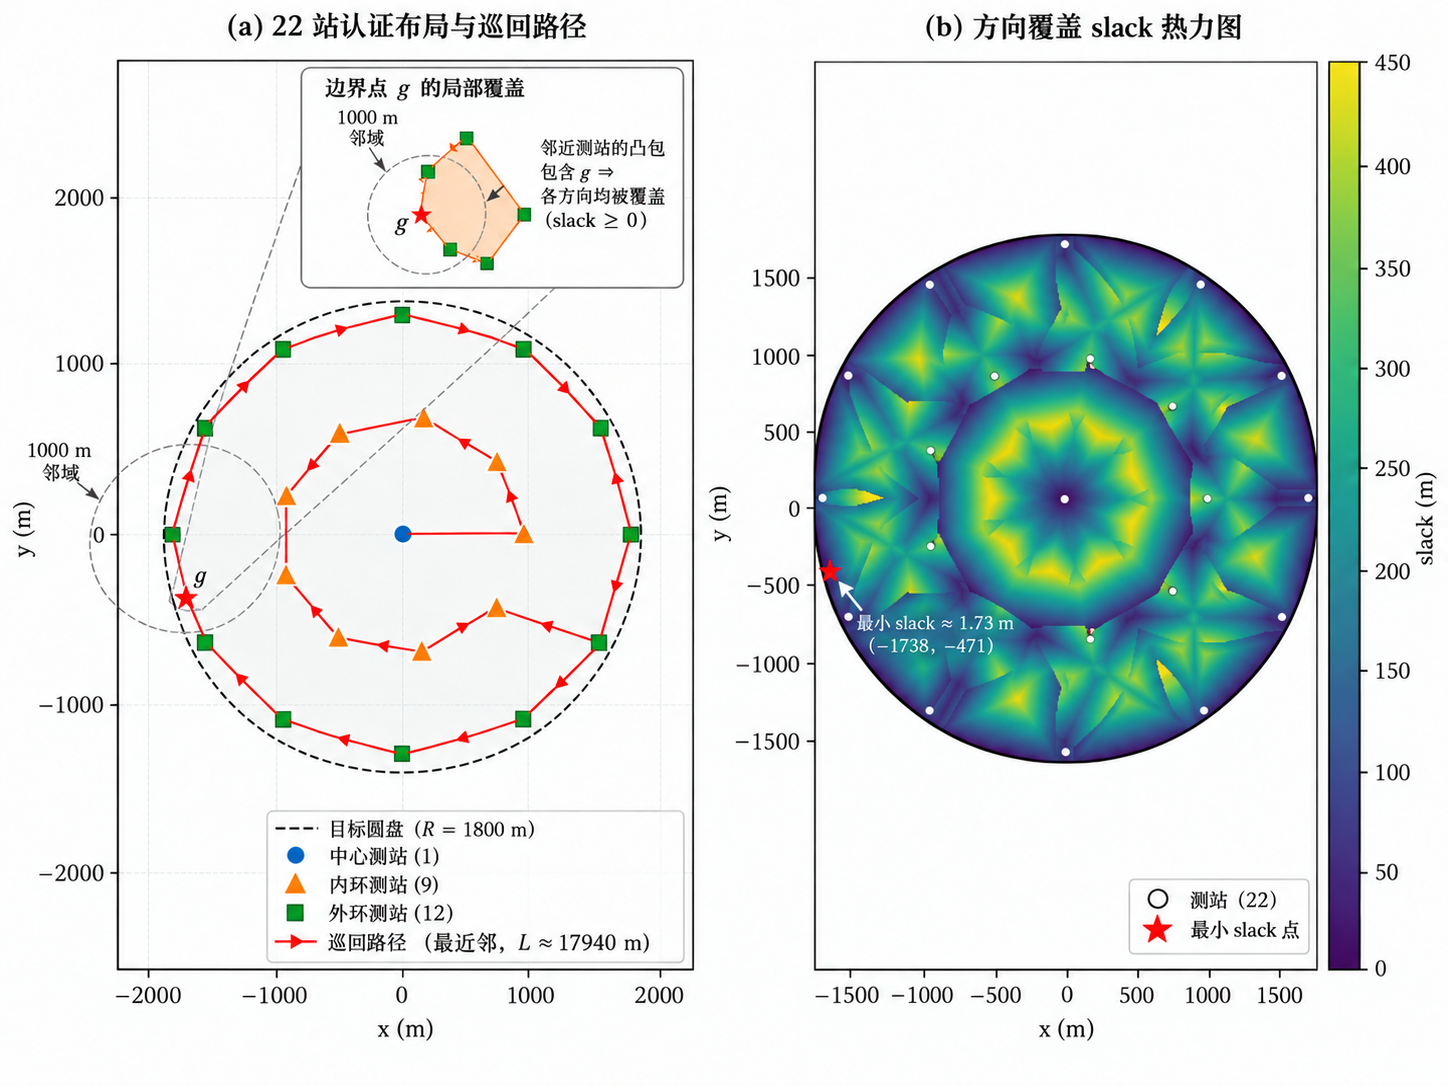
\includegraphics[width=\textwidth]{figures/fig-q4-layout.png}
  \caption{$22$ 站布局的方向覆盖证书}\label{fig:q4-layout}
\end{figure}

\subsection{在线层：选择性测量、有界等待与认证条带覆盖}\label{sec:q4:online}

第四问的定位层与第三问共用\cref{sec:q3:loc}的可行域递推与目标圆外包，但去掉\cref{thm:nosignal}的圆盘排除。在此基础上加入下列针对定向源的改进。

\paragraph{选择性重测.}

到达一个测站后，未发现的频道必须全部检测（这是终止证明的要求，不可省略）；但对已发现的频道，重复测量常常价值很低。设当前站为 $s$、目标可行域为 $P_c$，只有同时满足
\begin{equation}\label{eq:selective}
  \dist(s,P_c)\le950\mmet
  \quad\text{且}\quad
  \Bigl(\sin\widehat\psi\ge0.3\ \ \text{或}\ \ \min_{p\in\mathcal P_c}\|s-p\|\ge300\mmet\Bigr)
\end{equation}
时才重测，其中 $\widehat\psi$ 是以 $c_*(P_c)$ 为顶点、由已有采样点与 $s$ 张成的估计交会角，$\mathcal P_c$ 为已有采样点集。已经可以认证清除或已收到 \texttt{near} 的目标直接跳过。

\paragraph{有界等待与圆心补测.}

若某目标只有一条方位线，而后续巡站路线上正好有测站能提供第二条方位线（距可行域不超过 $950\mmet$），就可以推迟处理，等这次顺手可达的观测，省下一趟专程往返。为防止无限等待与错误等待，设了三重限制：只等一次；首次发现点距当前位置超过 $1400\mmet$ 时不等；在目标圆之外首次发现的目标不等——外环站能首次发现它，多半意味着该源朝外发射，后续站往往全部落在天线背面。

补测精化与第三问同理，只是阈值更紧：$\mecr\in(20,150]\mmet$ 时先走到 $c_*(P_c)$ 补测一次，若仍不够则沿新方位的垂线横移 $60\mmet$ 再补一次。

\paragraph{认证条带覆盖.}

$25\mmet$ 方格兜底（\cref{eq:grid}）只利用了清除圆的内接正方形，面积利用率为 $2/\pi\approx63.7\%$。本文改用沿首测方向的条带矩形覆盖：把 $P_c$ 沿 $\uvec{\theta}$ 切成宽 $w$ 的条，再在每条内沿横向切成高
\begin{equation}\label{eq:strip}
  h(w)=2\sqrt{r'^2-\left(\frac{w}{2}\right)^{2}},\qquad r'=r_c-0.1=19.9\mmet
\end{equation}
的矩形，取矩形中心为清除点。此时矩形四角到中心的距离恰为 $\sqrt{(w/2)^2+(h/2)^2}=r'<r_c$，由凸性整个矩形都落在清除圆内，覆盖性得证。$w$ 在 $\{1.25,1.5,1.7,1.9\}\times r'$ 中取；例如 $w=1.5r'=29.85\mmet$ 时 $h=26.32\mmet$，单点覆盖面积 $785.7\ \mathrm{m}^2$，比 $25\mmet$ 方格的 $625\ \mathrm{m}^2$ 高出 $25.7\%$。两种覆盖的对比见\cref{fig:q4-strip}。

\begin{figure}[!htbp]
  \centering


  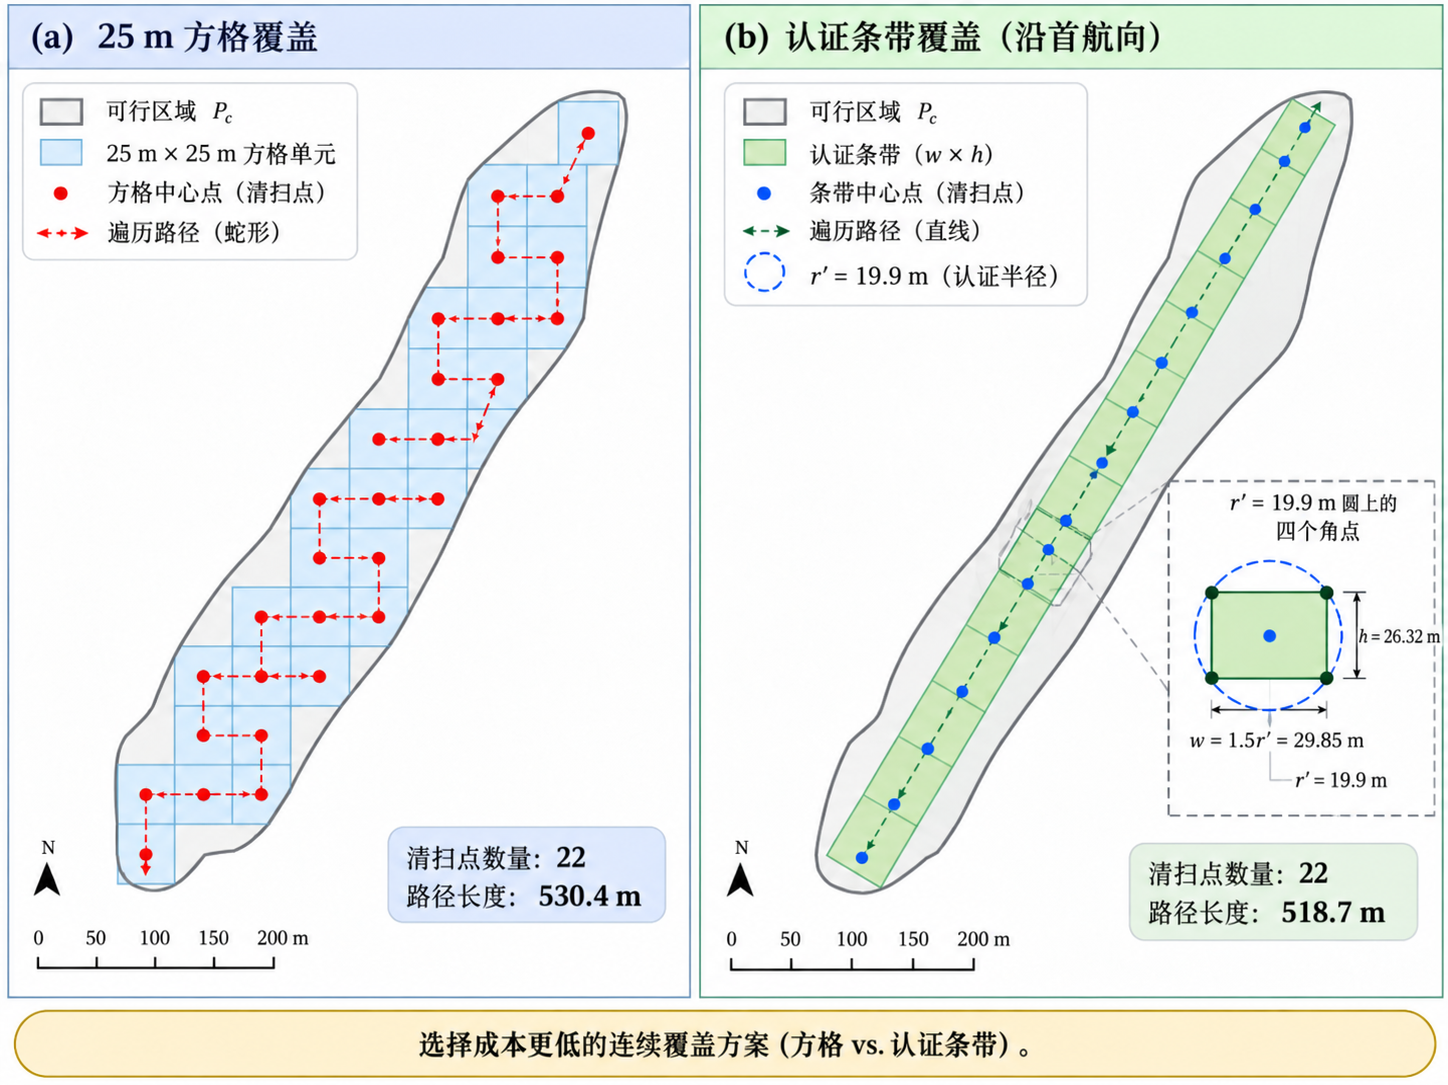
\includegraphics[width=0.9\textwidth]{figures/fig-q4-strip.png}

  \caption{两种具有连续覆盖证明的光学清除点列}\label{fig:q4-strip}
\end{figure}

\paragraph{扫描成本门控与即时清除.} 条带覆盖有时更慢：条带越宽，列数越少但每列越长，路径未必更短。因此算法同时生成方格路线与各个 $w$ 对应的条带路线，按
\begin{equation}\label{eq:routecost}
  \widehat C_{\rm route}=\frac{\|x_1-p_{\rm cur}\|+\sum_{i}\|x_{i+1}-x_i\|}{v}+|\{x_i\}|\cdot t_f
\end{equation}
取其中最小者。同样的比较也用在补测决策上：若估计的光学覆盖成本已不高于“走到补测点再测一次”的成本，就直接进入光学清除，跳过价值不足的补测。最后，收到 \texttt{near} 时在当前测站立即清除，而不等到本站扫描结束——真源就在 $5\mmet$ 之内，任何推迟只会增加往返。

\subsection{实验结果}

第四问历次结构性改进的配对实验见附录~\ref{app:sens}的表~\ref{tab:q4paired}，最后一次布局升级（$25\to22$ 站）的留出验证见\cref{tab:q4holdout}。

\begin{table}[!htbp]
  \caption{$25$ 站 $\to$ $22$ 站的留出验证（新种子 $2026100000$ 起，与全部开发种子不重叠；$220$ 例全部清除）}
  \label{tab:q4holdout}\centering
  \begin{tabular}{lcccccc}
    \toprule[1.5pt]
    场景 & 案例数 & $25$ 站均值 & $22$ 站均值 & $25$ 站 $\mathrm{P}_{95}$ & $22$ 站 $\mathrm{P}_{95}$ & $22$ 站更快 \\
    \midrule[1pt]
    随机       & $100$ & $494.5$ & $478.4$ & $675.5$ & $659.6$ & $73/100$ \\
    边界向外   & $30$  & $588.7$ & $557.9$ & $725.5$ & $683.8$ & $24/30$ \\
    最小接收半径 & $30$ & $517.0$ & $502.7$ & $677.0$ & $611.1$ & $20/30$ \\
    全部定向   & $30$  & $606.1$ & $574.9$ & $776.5$ & $726.3$ & $26/30$ \\
    圆心聚集   & $30$  & $450.9$ & $431.1$ & $598.2$ & $568.8$ & $28/30$ \\
    \bottomrule[1.5pt]
  \end{tabular}\\[2pt]
  \footnotesize 按源数分层（随机集）：$10$ 源 $666\to642$，$13$ 源 $491\to475$，$16$ 源 $361\to346$（虚拟秒/源）。
\end{table}



\cref{tab:q4holdout}显示 $22$ 站在五类场景的均值与 $\mathrm{P}_{95}$ 上都优于 $25$ 站，最困难的“边界向外”“全部定向”改善最明显（$30.8$ 与 $31.2\msec/$源）；但逐例表现有涨有跌，个别案例因发现顺序改变而变慢。本文保留的是“均值与分位数改善、清除率保持 $100\%$”这一较弱但站得住的结论（典型局轨迹与逐例配对见\cref{fig:q4-track}）。

\begin{figure}[!htbp]
  \centering
  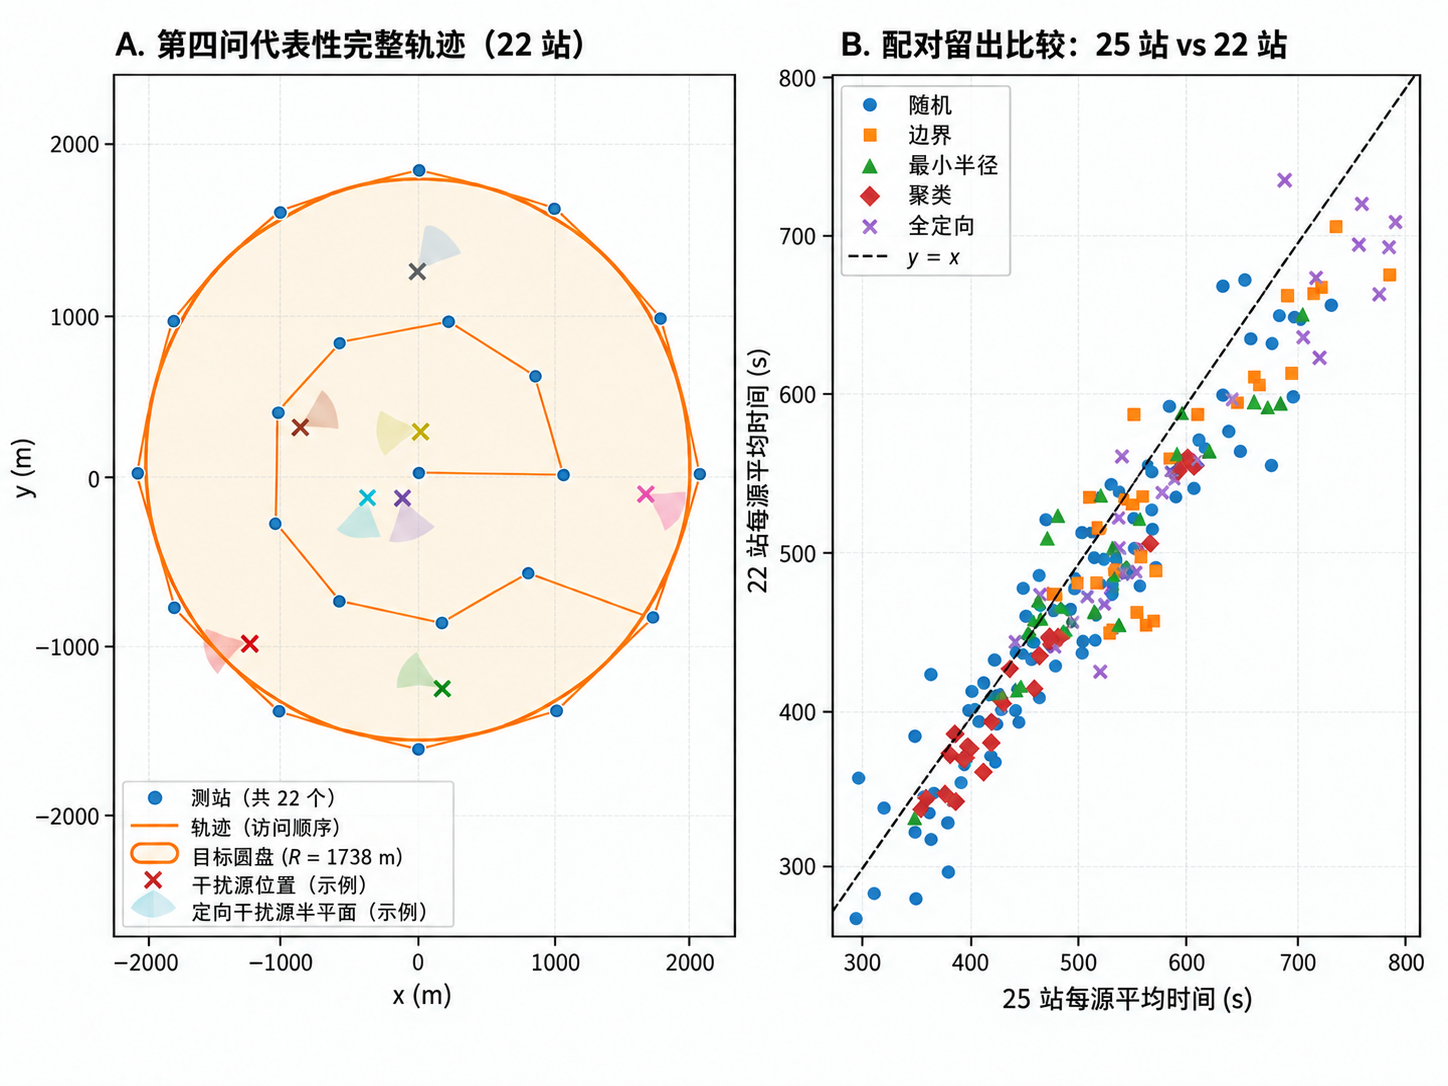
\includegraphics[width=0.9\textwidth]{figures/fig-q4-track.png}
  \caption{第四问典型局的行走轨迹与 $25$ 站／$22$ 站逐例配对}\label{fig:q4-track}
\end{figure}

\subsection{被否决的改进路线}

本文另试过七条改进路线（绕行代价阈值调度、价值门控裁剪重复测量、运行时动态跳站等），均完成完整配对实验但未获稳定收益，完整记录见附录~\ref{app:ablation}的\cref{tab:q4reject}。反复出现的教训是：\textbf{只盯着某个局部指标做优化，往往会在别处付出更大代价。}

\subsection{成本基准与“放弃保证”的代价}\label{sec:q4:lb}

把巡站、全站扫描与到达清除三项相加，得到第四问的成本基准；按源数分层，官方演练比该基准高 $6\%\sim11\%$。需要强调这是一个经验构造，用于判断“现有方案是否已接近一条合理的成本底线”。若放弃覆盖保证，用 $40$ 万个随机定向源做蒙特卡洛估计：$16$ 站时每局期望漏检 $0.14$ 个，约七局就有一局清除率低于 $100\%$；按“清除率是硬约束”的准则，这些方案一律不采用。完整的基准公式、分层表与风险表见附录~\ref{app:fixed}。

\paragraph{本问小结.} $22$ 站布局通过细／粗两次凸包检查，$220$ 例留出与 $70$ 局演练全部清除。需强调：\textbf{$22$ 是本文找到并认证过的最小站数}（其最优性尚未证明）。
